% Nome do Anexo
\chapter{Published Paper}
\vspace{-1.9cm}

Article entitled \textbf{A Systematic Mapping of Autonomous Vehicle Prototypes: Trends and Opportunities}, published in \textbf{IEEE Transactions on Intelligent Vehicles} in 2023.

The paper discusses the evolution of autonomous driving vehicles (ADVs) and aims to identify trends and opportunities in the development of these prototypes. Using a systematic mapping study, the paper analyzes 68 selected publications from a set of 548 papers. It provides insights into the hardware, software, and sensor architectures used in both real-size and miniature ADV prototypes. The mapping identifies key trends, technologies, and research opportunities, aiming to support researchers and developers in designing efficient ADVs.

\includepdf[pages=-, pagecommand={}]{pos-texto/IEEE_TIV.pdf}

% Nome do Anexo
\chapter{Published Paper}
\vspace{-1.9cm}

Article entitled \textbf{Hierarchical Heterogeneous Cluster Systems for Scalable Distributed Deep Learning}, published in \textbf{2024 IEEE 27th International Symposium on Real-Time Distributed Computing (ISORC)} in 2024.

Distributed deep learning framework tools should aim at high efficiency of training and inference of distributed exascale deep learning algorithms. There are three major challenges in this endeavor: scalability, adaptivity and efficiency. Any future framework will need to be adaptively utilized for a variety of heterogeneous hardware and network environments and will thus be required to be capable of scaling from single compute node up to large clusters. Further, it should be efficiently integrated into popular frameworks such as TensorFlow, PyTorch, etc. This paper proposes a dynamically hybrid (hierarchy) distribution structure for distributed deep learning, taking advantage of flexible synchronization on both centralized and decentralized architectures, implementing multi-level fine-grain parallelism on distributed platforms. It is scalable as the number of compute nodes increases, and can also adapt to various compute abilities, memory structures and communication costs.

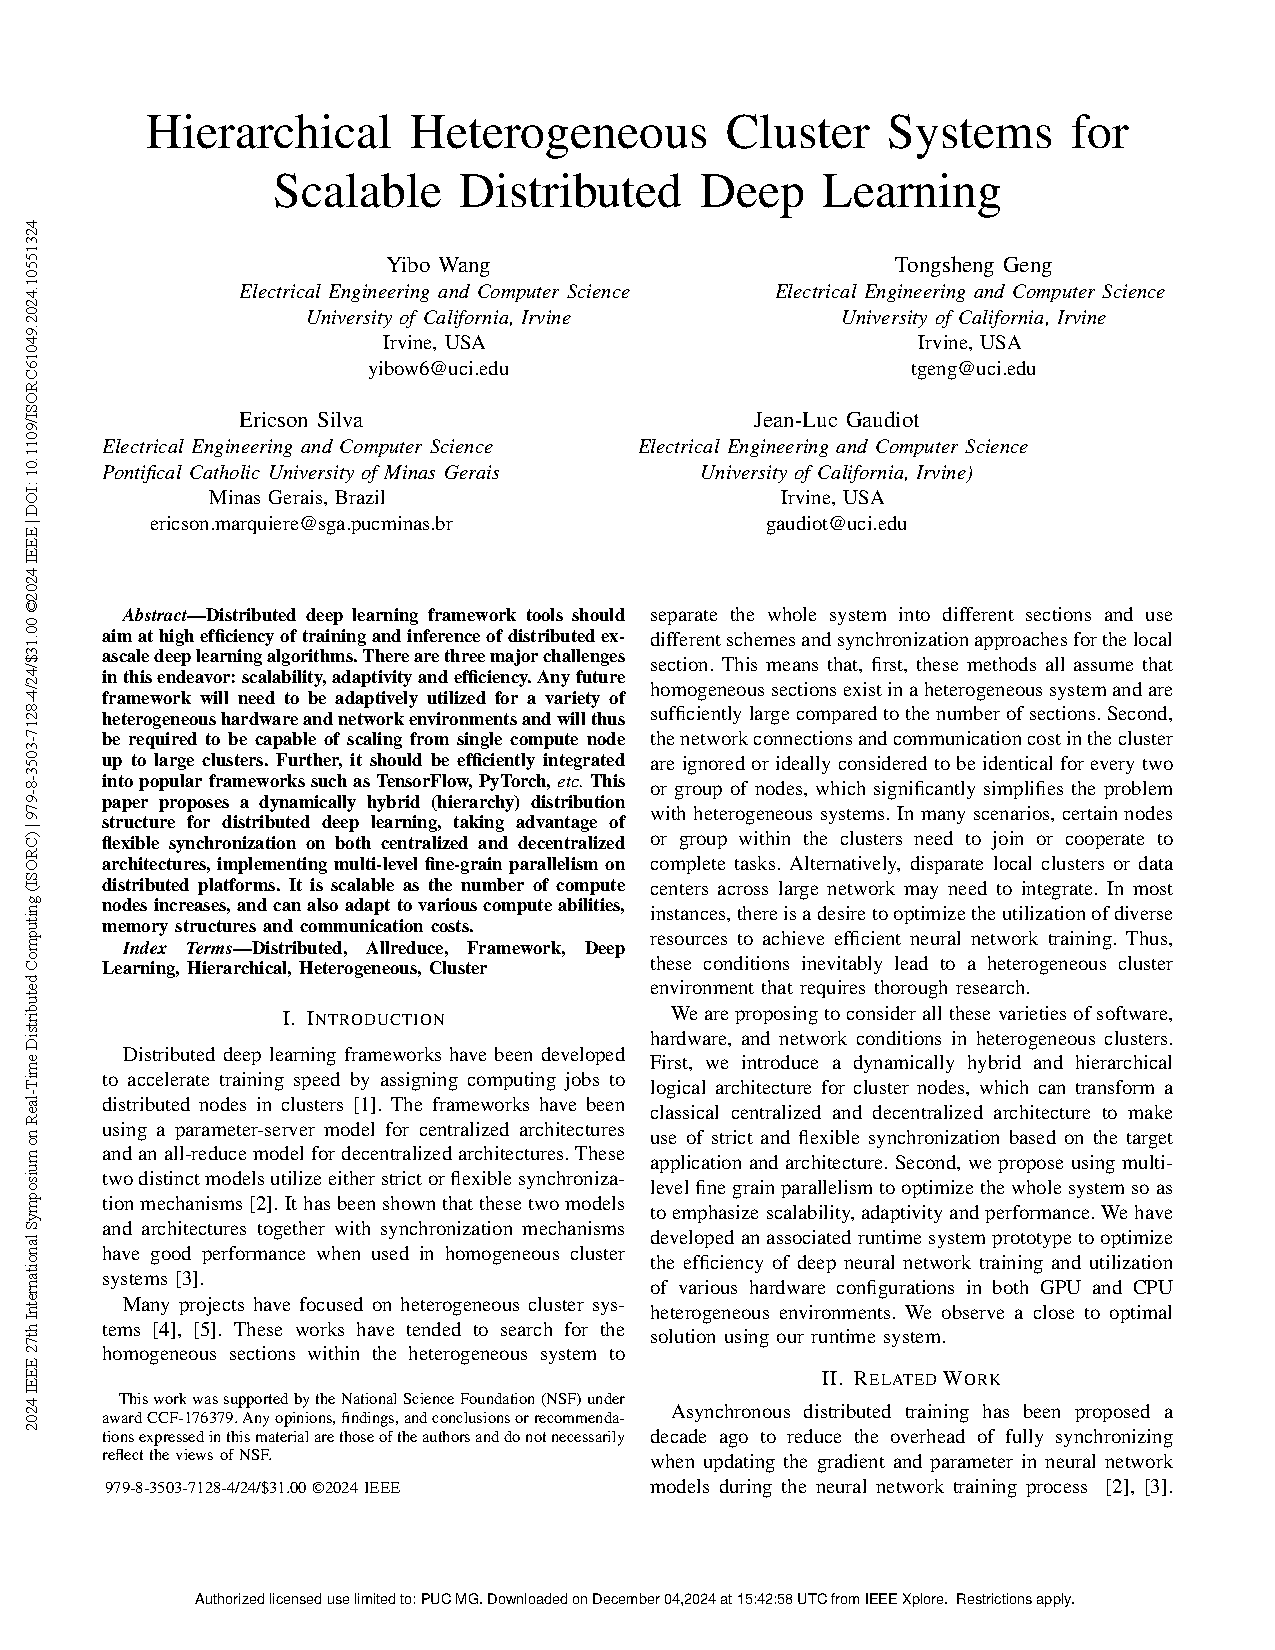
\includepdf[pages=-, pagecommand={}]{pos-texto/IEEE_ISORC}

\chapter{Accepted Paper}
\label{anexo-accepted}
\vspace{-1.9cm}

Article entitled \textbf{Task Scheduling for Autonomous Vehicles with Heterogeneous Processing via Integration of the CARLA Simulator and StarPU Runtime},accepted for publication in \textbf{IEEE International Conference on Consumer Electronics (ICCE)}, with a presentation scheduled for January, 2025.

The paper presents an innovative approach that integrates the CARLA simulator with the StarPU runtime system to optimize task scheduling in autonomous driving vehicles. By combining CARLA's detailed simulation capabilities with StarPU's flexible task management, the study explores efficient scheduling strategies for ADV perception and localization tasks using heterogeneous processing resources (CPU and GPU). The results indicate improvements in ADV performance, demonstrating the practicality of this integration for testing and optimizing task scheduling in realistic simulation environments.

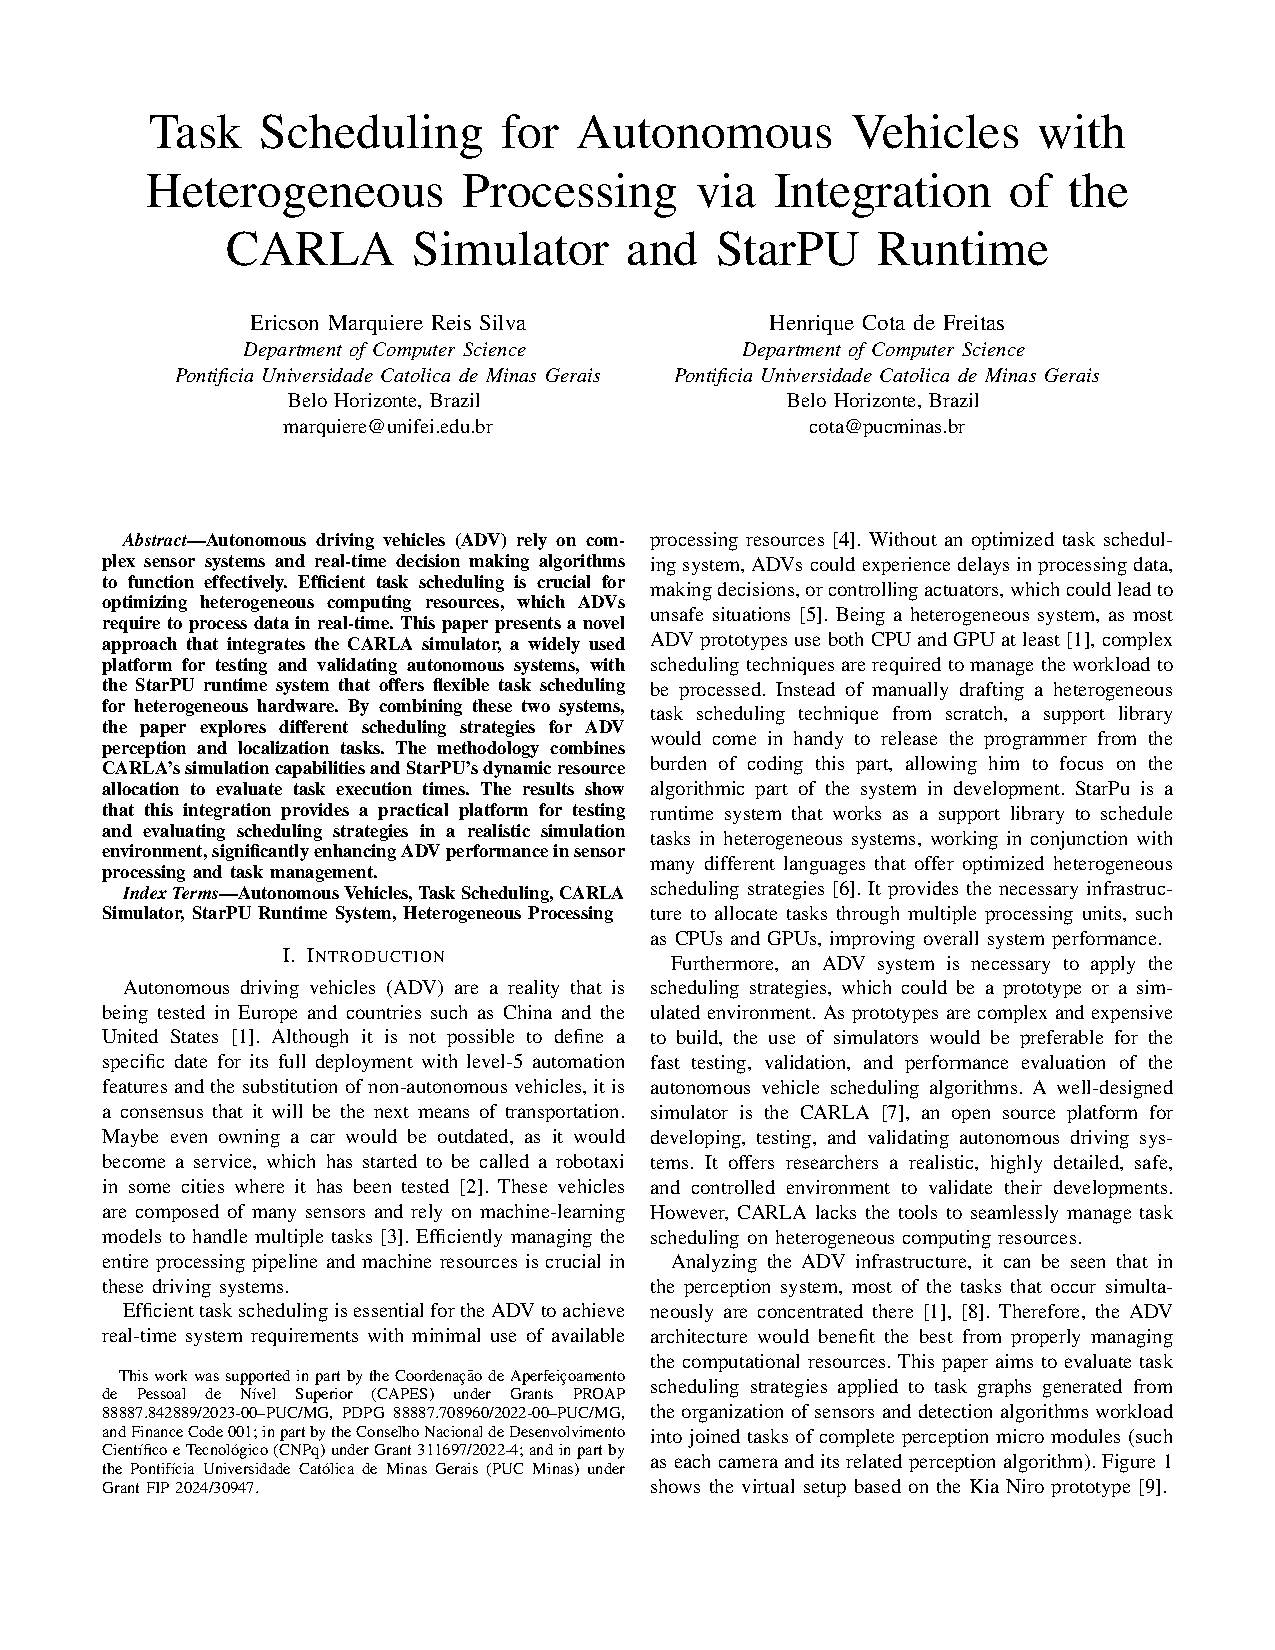
\includepdf[pages=-, pagecommand={}]{pos-texto/IEEE_ICCE.pdf}


